\documentclass[a4paper,12pt]{article}
\usepackage{graphicx}
\usepackage{longtable}
\usepackage{booktabs}
\usepackage{array}
%\usepackage{rotating}  % for sideways table
\usepackage[utf8]{inputenc} % Required for inputting international characters
\usepackage[T1]{fontenc} % Output font encoding for international characters
%\usepackage{fancyhdr} % Load the fancyhdr package
\usepackage[margin=1in]{geometry} % Optional, to control page margins
\usepackage{xcolor} % to determine colors
\usepackage[
    backend=biber,
    maxnames=2,
    style=authoryear,
    date=year]{biblatex} % Use the bibtex backend with the authoryear citation style (which resembles APA)
\usepackage{hyperref}
\hypersetup{colorlinks,
citecolor=teal,
linkcolor=cyan,
urlcolor=olive
}

% load references
\addbibresource{ms_crete_soil.bib}
% Adjust bibliography font size
\renewcommand*{\bibfont}{\small} % Use \footnotesize, \small, or other sizes
% title
\title{Meta-analysis of island soil microbiome reveals soil health indicators}
% authors
\author{
Savvas Paragkamian\textsuperscript{1,2,\dag, \P},
Johanna B. Holm\textsuperscript{3\dag},
Haris Zafeiropoulos\textsuperscript{4}, \and
Christina Pavloudi\textsuperscript{5},
Christos A. Christakis\textsuperscript{1}, \and
Ioannis Antoniou\textsuperscript{8},
Giorgos Kotoulas\textsuperscript{2},
Panagiotis F. Sarris\textsuperscript{1,8}, \and
Lynn Schriml\textsuperscript{3},
Evangelos Pafilis\textsuperscript{2, \P}
}
\begin{document}

\maketitle

\begin{center}
\textsuperscript{1} Department of Biology, University of Crete, Voutes, 70013, Crete, Greece \\
\textsuperscript{2} Institute of Marine Biology, Biotechnology and Aquaculture (IMBBC), Hellenic Centre for Marine Research (HCMR), Gournes, 71500, Crete, Greece \\
\textsuperscript{3} University of Maryland School of Medicine, Institute for Genome Sciences \\
\textsuperscript{4} Department of Microbiology, Immunology and Transplantation, Rega Institute for Medical Research, KU Leuven, Leuven, Belgium \\
\textsuperscript{5} European Marine Biological Resource Centre, Paris, France \\
\textsuperscript{6} Department of Mathematics, Aristotle University of Thessaloniki, 54124, Thessaloniki, Greece \\
\textsuperscript{7} Department of Environmental Science and Technology, University of Maryland, Baltimore, USA \\
\textsuperscript{8} Institute of Molecular Biology and Biotechnology, Foundation for Research and Technology-Hellas, 714 09 Heraklion, Crete, Greece
\end{center}
\vspace{1em}

\noindent\textsuperscript{\dag} These authors contributed equally as first authors. \\
\noindent\textsuperscript{\P} Corresponding authors: \texttt{s.paragkamian@hcmr.gr}, \texttt{pafilis@hcmr.gr}

\begin{abstract}


\end{abstract}

\noindent\textbf{Keywords:} soil microbiome, networks, island, Crete, spatial data, remote sensing, data integration, FAIR data\\

\noindent\textbf{Highlights}

\begin{itemize}
    \item Data integration of soil in Crete revealed vulnerable ecosystems
\end{itemize}


\section{Introduction}\label{intro_idea}


In this study we ask: 

Are there any alarming soil health signals in Crete derived from the rich open data?
To further support our case we use the
Island Sampling Day (ISD) soil microbiome data \parencite{holm2025first},
as a large scale bacterial study, to gain insights about the differences of the
microbiome communities across land use, aridity and microbial functional categories in Crete island.

\section{Materials and Methods}\label{integration_methods}


\subsection{Health assessments of Island Sampling Day Crete}\label{isd_data}

This study uses the ISD Crete data that have been deposited
in the European Nucleotide Archive (ENA) at EMBL-EBI under accession number PRJEB21776.
The raw sequences (fastq files) and metadata (xml files) were downloaded with custom scripts using the ENA API \parencite{ocathail2024the-european}.
Specific information regarding the ISD sampling, DNA extractions, PCR and sequencing
protocols are discussed here \parencite{holm2025first}.

Amplicon Sequence Variants were inferred using DADA2 \parencite{Callahan2016} for 
filtering, denoising and chimeric reads removal. Normalisation of the reads at 10000 reads
across samples was implemented with the SRS R package \parencite{Beule2020}. Samples
with less than 10000 reads were removed. ASVs were assigned to taxonomy using 
DADA2 with Silva 138 taxonomy \parencite{quast_silva_2013}.
PEMA was used for OTU inference based on VSEARCH \parencite{zafeiropoulos2020pema} with Silva 132 taxonomy.

The numerical ecology analyses, e.g diversity indices, NMDS, PERMANOVA, were calculated
with the vegan R package \parencite{oksanen2024vegan}.
For PCoA ordination the ape R package \parencite{Paradis2004} and UMAP python library \parencite{mcinnes2018umap-software}.
U-CIE R package was used for coloring 3 dimensional data \parencite{Koutrouli2022} to 
visualise the $\beta$ diversity differences of samples on the map.
Taxa functional annotation was implemented with the manually curated FAPROTAX database
with the accompanied python script \parencite{loucaDecouplingFunctionTaxonomy2016}.
%The network inference was facilitated with FlashWeave 0.19.2 \parencite{Tackmann2019}.
%To use FlashWeave we reduced 
%the abundance table of the ASVs to keep the ones at the genus or species level.
%The subsequent network analyses were carried out
%with the igraph R package \parencite{Csardi2006}. 
The differential abundance analysis was facilitated with the ANCOM-BC2 R package \parencite{Lin2023} using the 
different spatial layers from the maps section.

\subsection{Tools and code}\label{Coding environment}
The working environment had Python 3.11.4, R version 4.3.2 \parencite{rcoreteam}.
In terms of managing spatial data, geometry, and transformations, the following
R packages were used:
sf package version 1.0-14 \parencite{Pebesma2023}, for polygons, and the terra
package version 1.7-55 \parencite{hijmans2024terra}, for rasters.
Visualisation was implemented with ggplot2 \parencite{wickham_ggplot2_2016} and pheatmap \parencite{Kolde2019}.
Taxon names resolve and taxonomic classification was facilitated by taxize R package \parencite{chamberlain_taxize_2013}.
Finally, computations were performed on HPC infrastructure of HCMR \parencite{zafeiropoulos_0s_2021}.
Scripts about data integration are available in
\href{https://github.com/savvas-paragkamian/crete-idea.git}{Crete data integration repository}.
Scripts about the soil health assessment are available in 
\href{https://github.com/savvas-paragkamian/crete-soil-health.git}{Crete soil health assessment repository}.

\section{Results and Discussion}\label{crete_idea_results_discussion}


The retrieval of metagenomic data revealed that multiple 
seminal worldwide soil microbiome projects include one or two topsoil
samples from Crete \parencite{Vasar2022, Labouyrie2023, Bahram2018, Orgiazzi2018}.
Some have focused on soil fungi \parencite{Mikryukov2023, Davison2021, Tedersoo2021}
and other soil eukaryotes \parencite{Aslani2022}.
The Koiliaris Critical Zone Observatory \parencite{tsiknia2014environmental}, also a LTER,
is the most thoroughly studied soil ecosystem of the island. 
Whereas the Island Sampling Day (ISD) project \parencite{holm2025first}
is the most comprehensive soil microbiome study of Crete featuring 144 soil samples 
from 72 distinct locations. 
This sampling, denser comparing continental studies with 0.017 samples per km\textsuperscript{2},
makes possible comparison across the landscapes of the island.

ISD was organised by the Genome Standards Consortium \parencite{Field2011} and the Hellenic Centre for Marine Research
as a single day event to avoid seasonality effects and to create a snapshot of soil microbiome.
ISD is an amplicon 16s rRNA marker gene study with published open data with immediate release at PRJEB21776 ENA project,
alongside rich metadata (location coordinates, DNA concentration,
total nitrogen, total nitrogen, water content, total organic carbon) \parencite{holm2025first}.

\subsubsection{Inference and taxonomy}

All available ISD sequences and metadata were downloaded from ENA, which resulted in 140 samples. 
From the reported 144 samples, there was one sample missing, possible due to upload errors and other 3 that resulted to low DNA.
In total, samples had 60.6 million reads and the subsequent filtering and quality control (Ns and chimeric sequences removal and denoising)
reduced the size to 33.3 million reads. Two samples were excluded from the analysis because they had
fewer than 10000 reads. 

Denoising with, DADA2 resulted in 216,360 ASVs (2,704 unique
taxa; 1123 ASVs at species level and 1059 at genus level). OTU inference with
PEMA (VSEARCH) resulted in 13,285 OTUs; 2319 at family level and 1920 at genus level, Table \ref{table:asv_taxonomy}.


About 98\% of ASVs occur in 2 samples or less as shown in Figure \ref{fig:isd_microbiome}A.
Hence, finding the prevalent ASVs is no trivial in soils of Crete.

\begin{table}[]
    \caption{Taxonomic depth of ASVs and OTUs of the ISD microbiome.}%
\begin{tabular}{@{}lllll@{}}
    \textbf{Classification} & \textbf{Total ASVs}    & \textbf{Total (ASV) taxa} & \textbf{Total OTUs} & \textbf{Total (OTU) taxa}\\
Kingdom              & 1974         & 2                & 284        & 2               \\
Phylum               & 4034         & 33               & 121        & 15              \\
Order                & 38517        & 193              & 1224       & 135             \\
Class                & 24157        & 83               & 978        & 62              \\
Family               & 71355        & 287              & 2319       & 218             \\
Genus                & 90137        & 1166             & 1920       & 582             \\
Species              & 9120         & 1338             & 44         & 43              \\
Total                & $\sim$239000 & 3102             & 6890       & 1057            
\end{tabular}
\label{table:asv_taxonomy}
\end{table}

There are 25 specialist taxa (present in samples < 10 and mean relative
abundance > 0.003) and 146 generalist taxa (samples > 120), Figure \ref{fig:isd_microbiome}A.
The representative Phyla, i.e the Phyla with higher than 5\% presence in all samples, are:
Actinobacteriota, Proteobacteria, Chloroflexi, Acidobacteriota,
Bacterodota and Planctomycetota, Figure \ref{fig:isd_microbiome}B.
Actinobacteriota and Proteobacteria in particular are present in all samples with 
more than 50\% joined relative abundance, 36\% and 19.5\% respectively.
Acidobacteriota aren't amongst the top phyla in 11 samples, 9 of them are beach
ecosystems.


Networks specialists generalists \parencite{Barberan2012}
Positive and negative in soils \parencite{Liu2024}

Additional notable mentions of phyla are the Desulfobacterota which have specialist
role in the ERR3697703 sample from Richtis gorge. Gemmatimonadota appear mostly
in low carbon, dry samples and related with grazing.
The genus Deinococcus,
from the Deinococcota phylum, appears in 3 samples from sandy beaches with high relative abundance.
Apart from bacteria, there are two phyla of archaea in the ISD data, Thermoplasmatota and Euryarchaeota.
These occur in samples from Kolokytha islet, Agiofaraggo gorge and Schinaria beach, all in the 
beach environment. 

\begin{figure}[hbt!] 
    \centering\includegraphics[width=\columnwidth]{figures/fig_isd_microbiome.png}
    \caption[Island Sampling Day]{Soil microbiome diversity of Crete based on ISD data.}
    \label{fig:isd_microbiome}
\end{figure}


\subsubsection{Functions, associations and compositions}


Figure \ref{fig:soil_communities}. 


\begin{figure}[hbt!] 
    \centering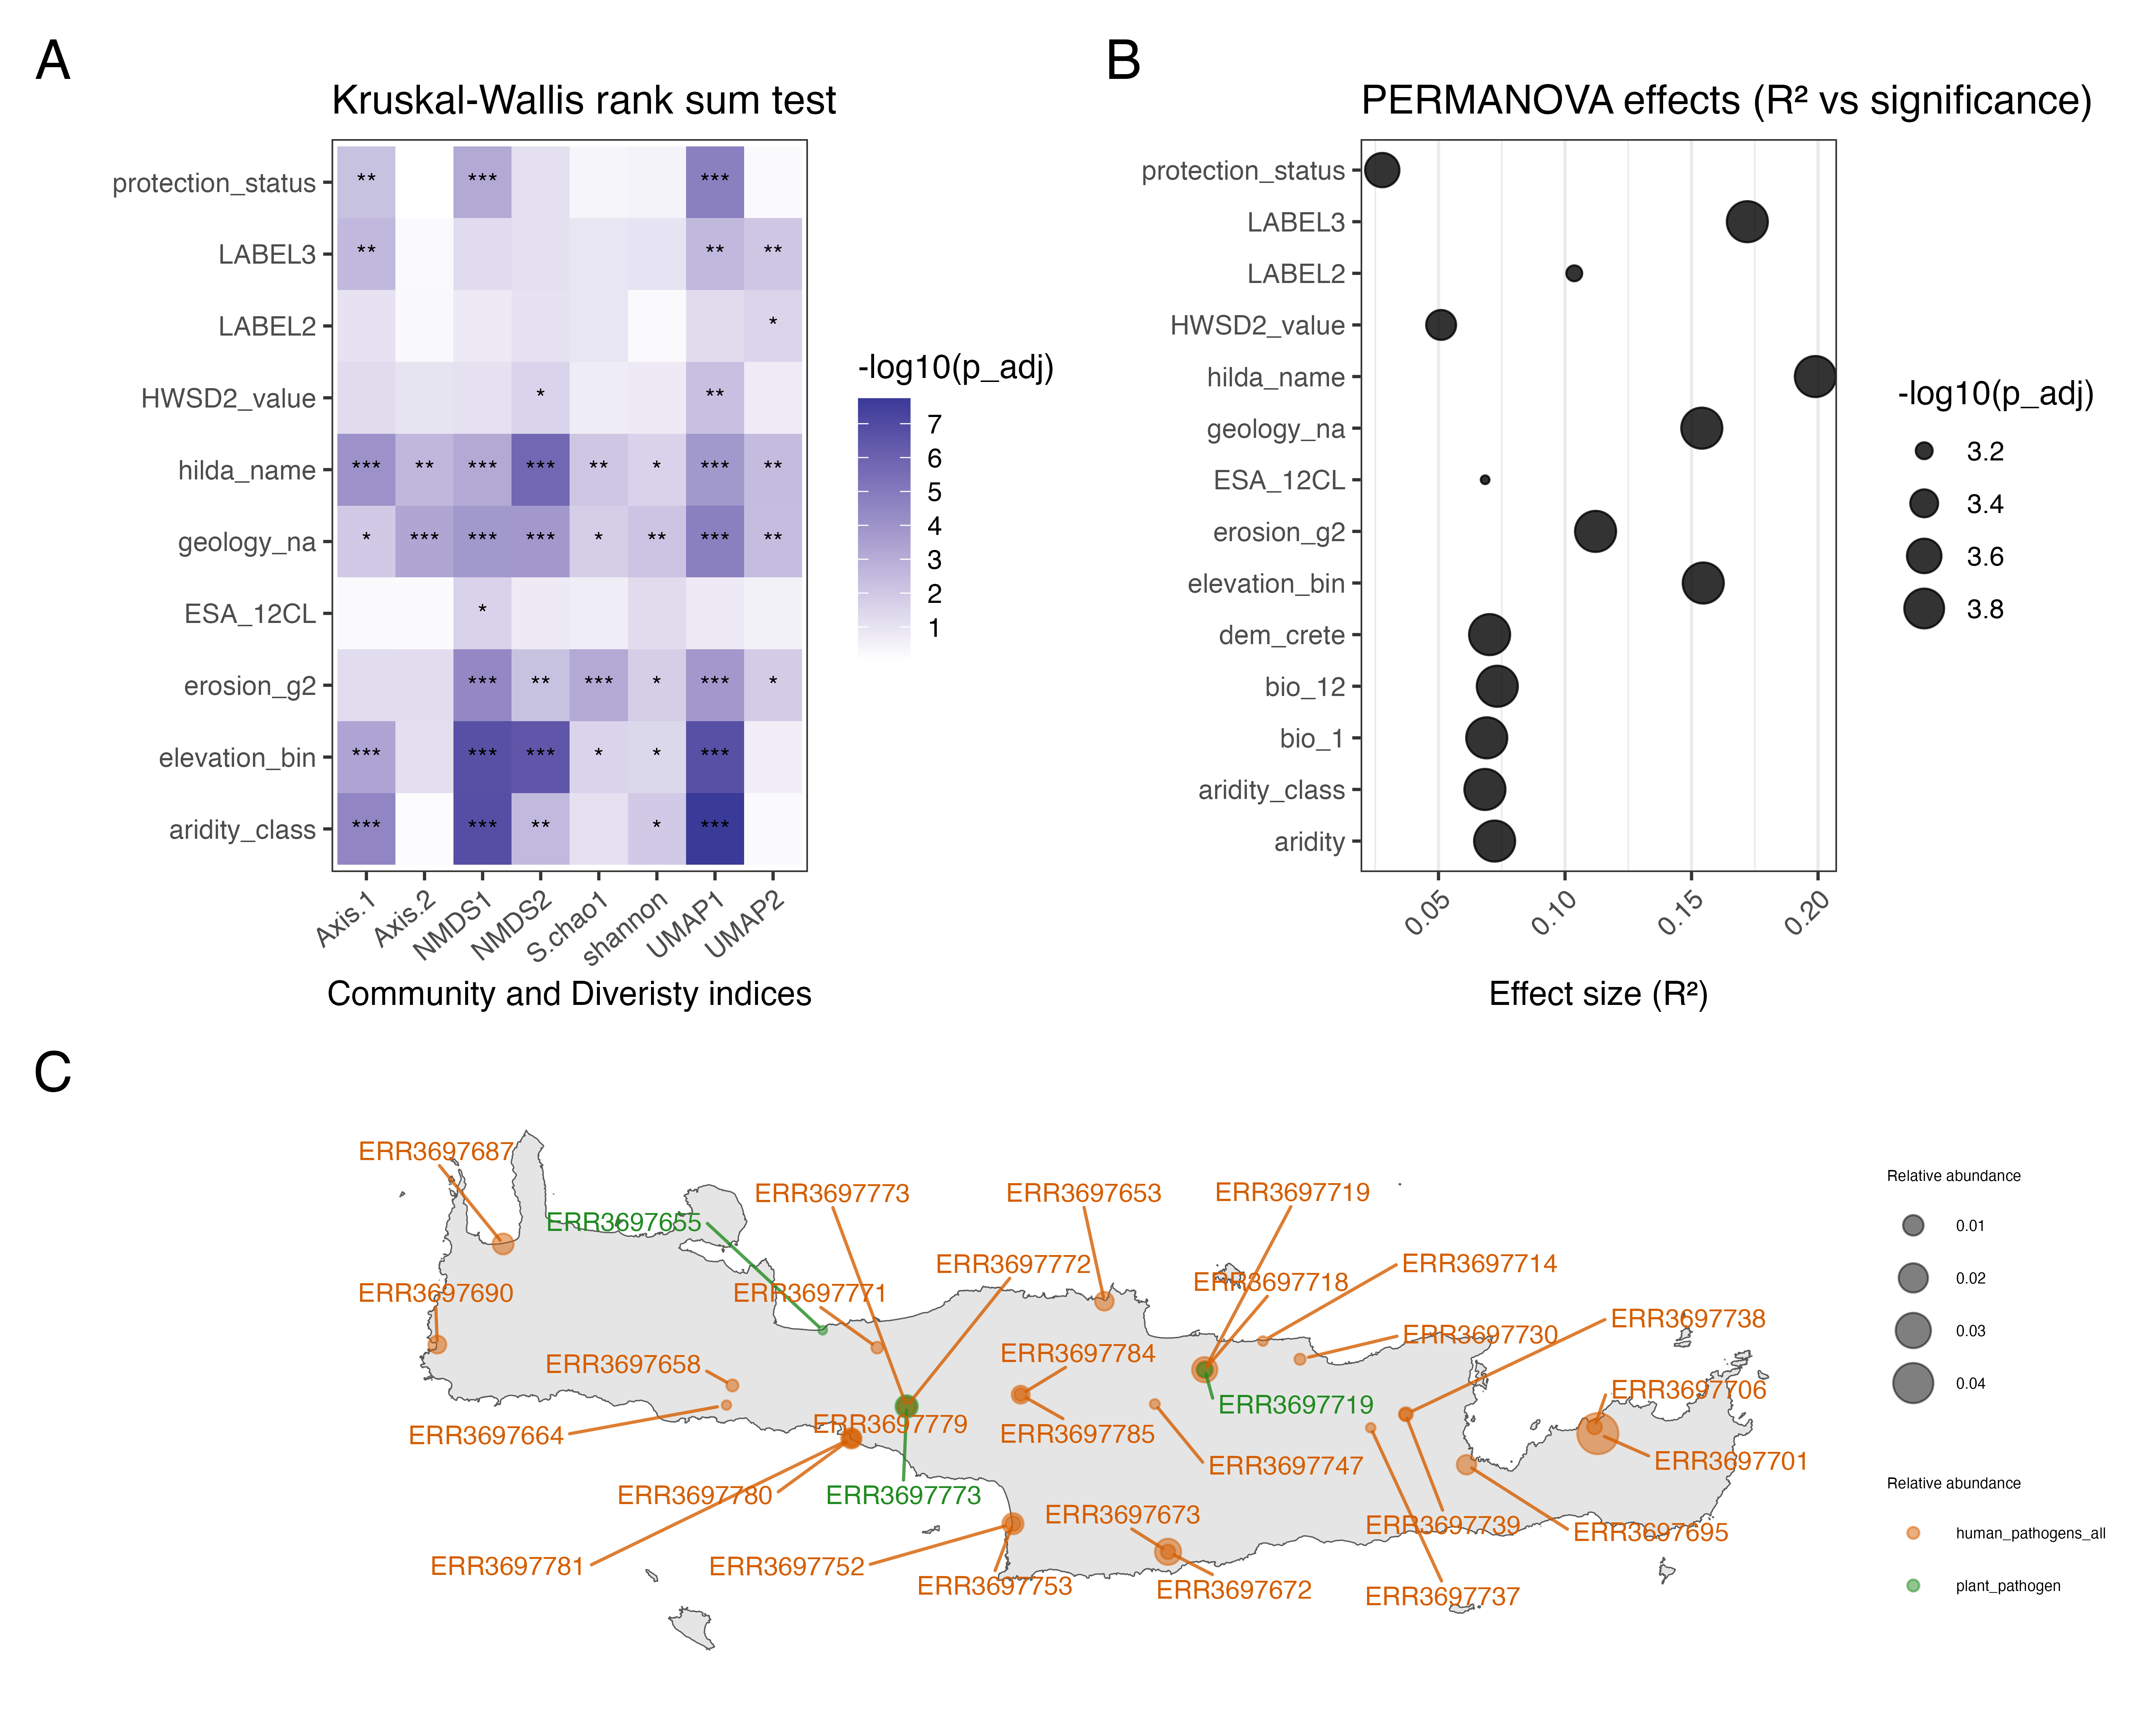
\includegraphics[width=\columnwidth]{figures/fig_isd_community_stats.png}
    \caption[Soil communities and maps]{Soil microbiome diversity of Crete based on ISD data. A. 
    B. PERMANOVA results of significance and effect size across different map layers.}
    \label{fig:soil_communities}
\end{figure}


Differential abundance.
Another important finding is the statistically significant presence of \textit{Rhodococcus equi} (pathogen of foal or similar)
in pastures. It is one of the most common causes of pneumonia in foals which
become infected by inhaling dust or soil particles contaminated with the bacterium.

Richtis gorge  \ref{fig:soil_abundance}.

Richtis gorge (highly popular) has alarmingly high values for human pathogens, sulfur respiration and
nitrate reduction. Even though this is derived from projections based on 
taxonomic informations it shows some trends.
This gorge has water all year long, rare in the gorges of Crete,
and is the highest touristic attraction of eastern Crete. Its' name means "throw" and 
there is a local rumor that people threw unwanted stuff throughout the centuries. 
Origins of the name is also possible to be from the waterfall, which in Crete dialect
is sometimes mentioned as "Rechtara", "Rechta" and "Richtis".
Nevertheless, it is an important freshwater ecosystem which, to my knowledge is not included in 
any protection regimen or legislation.
The prevalence of potential human pathogens in Richtis gorge are an alarming signal which needs to be further investigated.



\begin{figure}[hbt!] 
    \centering\includegraphics[width=\columnwidth]{figures/fig_isd_differential_abundance.png}
    \caption[Differential abundance]{Soil microbiome diversity of Crete based on ISD data.}
    \label{fig:soil_abundance}
\end{figure}

Functional predictions from taxonomic information can lead to logical fallacy and oversimplification. 
That is the case because the predictions are biased from reference genomes that are 
used to assign functions to microbial taxa. In addition, amplicon studies like ISD
cannot lead to certain results at the strain level and microbes are known for 
their high degree of functional gene exchange in the environment \parencite{douglas2020picrust2}. 
Early studies in soil metagenomics showed that deeper sequencing was needed to 
accurately predict functions especially in ecosystems with low biodiversity like deserts \parencite{fierer2012cross-biome}.
Reversely, functional groups when studied at the ecosystem level can be described 
without gene specific information because there is a correlation of function with taxonomy \parencite{loucaDecouplingFunctionTaxonomy2016}.
These projection can act as a preliminary assessment as shown in \textcite{Labouyrie2023}.
Even though amplicon studies in soil should be interpreted with caution \parencite{alteio2021} they 
can act as early warning signals towards public health concerns \parencite{banerjee2023Soil}.
Using amplicon studies to function prediction has limitations and metagenomics of total DNA is more accurate \parencite{matchado2024on-the-limits}.

Shotgun metagenomics and metatranscriptomics can unleash the functional potential of
topsoil along with other advancements like long reads sequencing. Higher resolution
samplings using grid system will enhance the resolution and also the resampling of
ISD sites in different time points will provide additional insights to the complex soil 
functions and expand the positive and negative associations in soils \parencite{Liu2024}.

\section{Conclusion}



\begin{table}[h!]
\centering
\caption{Summary of sequencing and quality filtering.}
\begin{tabular}{@{}ll@{}}
\textbf{Metric} & \textbf{Value}     \\
Samples         & 140                \\
Reads           & $60.6 \times 10^6$ \\
Ns              & $76.000$           \\
Filtered        & $50.1 \times 10^6$ \\
denoisedF       & $45.9 \times 10^6$ \\
denoisedR       & $48.5 \times 10^6$ \\
merged          & $35.0 \times 10^6$ \\
nonchim         & $33.3 \times 10^6$ \\
\end{tabular}
\label{tab:metrics}
\end{table}

Reads shorter than 445 bp or longer than 515 bp were fewer than
15,000.
Reads with unknown bases, Ns, were removed.
From the 140 samples retrieved from ENA, two samples were 
neglected because they had fewer than 10000 reads. Comparing with the ISD data
4 samples were missing, possibly due to upload errors.
Thus, 138 samples in total were included in the subsequent analysis.



\section{Data and Code}
Scripts about the soil health assessment are available in 
\href{https://github.com/savvas-paragkamian/crete-soil-health.git}{Crete soil health assessment repository}.
This repository contains all the necessary scripts for the microbiome data retrieval,
filtering and ASV inferrence, taxonomy assignment, data integration of spatial data, 
functional annotation and the subsequent analyses and visualisation.

\section{Competing interests}
No competing interest is declared.

\section{Author contributions statement}
Conceptualization: SP, EP, LS, JH;
Data curation: SP;
Formal Analysis: SP, JH, HZ;
Funding acquisition: SP, EP, PFS;
Investigation: SP, JH, HS, CP;
Methodology: SP, JH, HS, CP, CC;
Project administration: EP, LS;
Resources: SP, GK, EP;
Software: SP, JH, HZ;
Supervision: EP, LS, PFS, IA;
Validation: JH, CP, CC, HZ, PFS, LS, EP;
Visualization: SP;
Writing – original draft: SP, JH, HZ, CP;
Writing – review and editing: All authors.

\section{Acknowledgments}

\section{Funding}
SP was supported by the 3rd H.F.R.I. Scholarships for PHD Candidates (no. 5726) for his work.

\printbibliography[heading=bibintoc]
\end{document}
